\documentclass[a4paper]{article}

\usepackage{INTERSPEECH2015}

\usepackage[utf8]{inputenc}
\DeclareUnicodeCharacter{0181}{\Ɓ}
\DeclareUnicodeCharacter{0253}{\ɓ}
\DeclareUnicodeCharacter{018A}{\Ɗ}
\DeclareUnicodeCharacter{0257}{\ɗ}
\DeclareUnicodeCharacter{0198}{\Ƙ}
\DeclareUnicodeCharacter{0199}{\ƙ} 

\usepackage{graphicx}
\usepackage{amssymb,amsmath,bm}
\usepackage{textcomp}
\usepackage{hyperref}
\usepackage{subfigure}


\def\vec#1{\ensuremath{\bm{{#1}}}}
\def\mat#1{\vec{#1}}


\sloppy % better line breaks
\ninept

\title{Collaborative Annotation for Person Identification in TV Shows}

\makeatletter
\def\name#1{\gdef\@name{#1\\}}
\makeatother \name{\em Matheuz Budnik$^1$, Laurent Besacier$^1$, Johann Poignant$^2$, Hervé Bredin$^2$, Claude Barras$^2$,  \\
\textit{Mickael Stefas$^3$, Pierrick Bruneau$^3$, Thomas Tamisier$^3$}}

\address{$^1$Laboratoire d'Informatique de Grenoble (LIG), Univ. Grenoble Alpes, Grenoble, France \\
  $^2$LIMSI, CNRS - Orsay, France \\
  $^3$LIST, Luxembourg \\
  {\small \tt Mateusz.Budnik@imag.fr} 
}

\begin{document}
  \maketitle
  %
  \begin{abstract}
This paper presents a collaborative annotation framework for person identification in TV shows. The web annotation front-end will be demonstrated during the \textit{Show and Tell} session. All the code for annotation is made available on \textit{github}.
  \end{abstract}
  \noindent{\bf Index Terms}: multimodal person identification, collaborative annotation, active learning, data collection.

  \section{Introduction}
      \subsection{Context - Camomile project}
      % Mateusz: First as in "the first working version" or "first collaborative framework for such task"?
One of the objectives of the Camomile project \footnote{https://camomile.limsi.fr} is to develop a first prototype of a collaborative annotation framework for 3M (multimodal, multimedia, multilingual) data, in which the manual annotation is done remotely on many sites, while the final annotation is localized on the main site. 

        \vspace{-0.2cm}
 \subsection{Demo Content}
The demo presents our shot annotation interface for person identification in TV shows. The tool is supported by a web annotation front end, a server to centralize annotations as well as an active learning backend that are all described in section 2 of this paper. A dry run evaluation (small-scale annotation campaign) is also presented in section 3.
%As for the document structure, I would go the other way: first talk about the use case, and then about the interactive tools to support it. Else we have to talk about a problem that has not been already introduced.


      \section{Collaborative annotation framework}

%The ultimate purpose of the platform is to provide on demand overviews and details regarding the 3M data, and the associated automatic and manual annotations. 
In this paper, the focus is on manual annotations from multiple users. The proposed collaborative annotation framework follows a client/server architecture (see figure~\ref{fig:overview}). 

\begin{figure}[h]
 	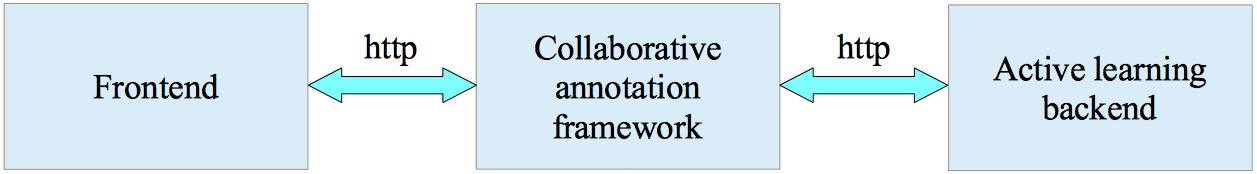
\includegraphics[width=0.45\textwidth]{overview.png}
	\caption{Overview of the Collaborative annotation using Camomile tools}
	\label{fig:overview}
\end{figure}

The frontend and backend parts can be seen as a client of the server part. The involved server-side technologies rely solely on exchanges via the HTTP protocol, facilitating the design of interoperable software components. The server focuses essentially on data and authentication management tasks, leaving the application logic to the client side. More details on the framework can be found at \cite{urlframework}.


      \subsection{Camomile server}

The server component provides access and basic CRUD operations (create, update, delete) for the resources, which can be any pieces of 3M data (corpus, media, layers and annotations). The web server is built on \textit{node.js} with \textit{express framework} and \textit{mongodb} as data storage solutions. The latest version of the server is available at \cite{urlserver}. 

        \vspace{-0.3cm}
      \subsection{Web annotation front-end}
        \vspace{-0.5cm}
%(présenter le front-end web et pointer sur le lien github précis - y passer plus de temps 

% Pierrick: from Mateusz' queue find a more illustrative example, i.e. with context annotation outside the current shot
\begin{figure}[h]
	\centering
 	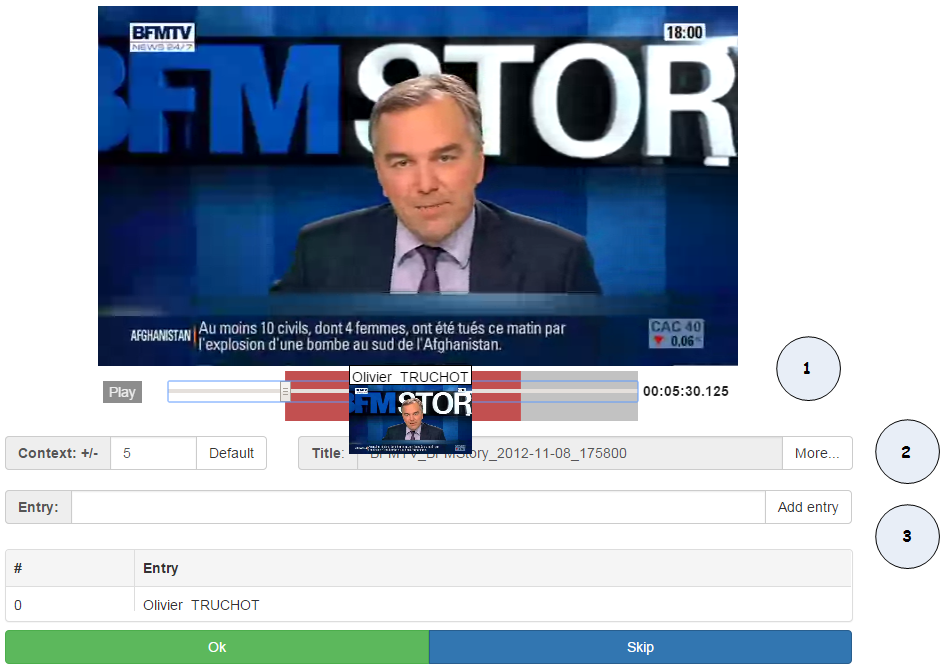
\includegraphics[width=0.4\textwidth]{camomile_ui-bis.png}
	\caption{Overview of the web front-end UI. 1) Video player displaying the shot to annotate and the synchronized \emph{context bar}. 2) The \emph{context bar} configuration and the metadata field. The latter displays the video title, and reveals additional details when activated. 3) The textfield to type the annotation. Multiple annotations are supported, and summarized in a table.}
	\label{fig:frontend}

\end{figure}

% Pierrick: during my trials for the demo video, I found that the annotation list was more annoying than anything else - I has to scroll everytime to do (next), whereas fitting in screen height would make things easier. Also, are multi-annotations to be supported?

An overview of the visual tool is shown in Figure~\ref{fig:frontend}. It uses display features provided by HTML5 and D3.js \cite{d3js}. The \textit{angular.js} framework \cite{angularjs} provides an efficient MVC framework to easily coordinate multiple views. The latest version of the tool is available at \cite{urlfrontend}.



Though there are two main use cases (see \ref{sec:shot} and \ref{sec:head}), components are mostly the same for both: the shot or the frame to annotate is displayed in a HTML5 video player and its metadata is shown under the player. The input of a set of annotations is supported by a textfield and a summary table. 

%Both use cases are part of an active learning loop. Each step outputs a selected list of annotations to be performed. Potentially multiple users connect to this list through the frontend, and process annotations in order. They can either validate an annotation of the current shot, or skip it if they feel unsure about it.


% Pierrick: do we talk about both head and shot annotation, or only shot?
%Laurent: we will remove head annotation if not enough space - because this is 2 pages maximum

\subsubsection{Annotate shot} \label{sec:shot}
        \vspace{-0.2cm}
In the first use case, a user has to name the speaker in the shot. The video player, restricted to the shot, allows to explore it at length.\\
Owing to the iterative nature of the active learning algorithm, the current speaker might have already been annotated elsewhere in the video. Seeking beyond the current shot might reveal such annotations. This obervation led to a \emph{context bar} being proposed, which provides the usual features of a seek bar, while revealing annotations performed in previous steps as overlay. A time span can be parametrized around the current shot, highlighted in red (see Figure \ref{fig:frontend}). Hovering over contextual annotations displays a tooltip containing a video thumbnail and the associated annotation.\\

        \vspace{-0.5cm}
\subsubsection{Annotate head} \label{sec:head}
        \vspace{-0.2cm}
% Pierrick: did not change anything here for now
The second one corresponds to giving the identity of a person appearing on screen. In that case, there is no need to scroll through the video, so only the correspong frame is dislayed to the user. As several persons can appear on screen, it is necessary to help users to figure out which one has to be identified. For this, a layer on the frame was added, on which a red square surronding the head of the person to name was drawn.\\


%Resp : LIST
        \vspace{-0.5cm}
      \subsection{Active learning backend}
        \vspace{-0.1cm}
%(présenter l'approche LIG - retraining and adaptation - et pointer sur le lien github précis - y passer plus de temps 

%Resp : Matheusz
In order to make the annotations provided by the users more relevant, an active learning system 
was developed. The approach can be described as an unsupervised active learning since no biometric models are trained and only speaker clustering is performed (ideally, each cluster corresponds to an individual person).  In this method a hierarchical clustering algorithm was used 
following the  approach presented in \cite{poignant2012unsupervised}.  The clusters consist of tracks: speech (based on speaker diarization),  face (the result of face tracking) or both in the case of multimodal clusters. In the latter case, the distance between tracks from different modalities is based on the output of a multilayer perceptron.

At each step of the algorithm, the user is presented with a set of tracks for annotation. Then, the clustering is refined when new annotations are introduced.
The label given to a particular track is propagated to the whole corresponding cluster. Next, a selection strategy is applied, which tries to verify the correctness of the annotated clusters or to label new ones.
More in-depth description of the method can be found in \cite{budnik2014automatic}.

%      \subsection{Compatibility with other annotation tools}
%voir si on ajoute une partie comme ça ou pas?
%%Mateusz: Does this refer to the whole system? Or just particular components?
%Resp : LIMSI
%


  \section{Dry run evaluation}
      \subsection{Use case : multimodal speaker annotation}
     
%décrire la tâche et les participants à l'expe

%Resp : Mateusz
A dry run annotation was done to evaluate the efficiency of the whole system. The task consisted of annotating speakers in videos. The speech tracks were extracted automatically following the approach presented in \cite{barras2006multistage}.
Each participant was given a video fragment corresponding to the time frame of a speech track and was asked to name the person speaking at the moment.
The user had also access to the whole video. Due to the nature of the videos (TV news broadcasts), most people were presented either by an overlaid text or by a spoken name.
 
      
      \subsection{Quantitative analysis}
 
9 persons were involved in the dry run. The annotations were done simultaneously and lasted for around 1.5 hours per user.
In this run only the speaker annotation scenario was tested. The corpus consisted of 62 videos from the REPERE dataset \cite{giraudel2012repere}, which included TV debates, news programs and parliamentary broadcasts among others.  During the run, a total of 716 speech tracks (81mn) were annotated. Additionally, 654 tracks (68mn) were marked as skipped (tracks which do not contain speech, but music, external noises, etc.). The median annotation time is equal to 10.8s. Additionally, because of the clustering present in the system, the annotations were propagated to the corresponding clusters. This produced a total number of 3504 labeled tracks (including the 716 annotated manually) with the total time equal to 7.81h. As a \textit{by-product}, the use of the multimodal clusters during the dry run enabled to get face annotation (1973 head annotations - 5.47h total). 

%After removing the outliers (for example: due to people leaving the annotation system for an extended period of time while still logged in) the average annotation time is 20.0s and the median is equal to 10.8s.


%The annotation obtained through propagation is not free of error, but could be re-annotated using our framework, this time in a verification (\textit{active cleaning}) scenario.


 
    
%stats présentés par Matheusz au meeting de Madrid

%Resp : Mateusz
  
        \vspace{-0.2cm}
     \subsection{Qualitative analysis}
        \vspace{-0.1cm}    

%Analyse des resultats du Survey

During the survey, participants had to fill a form to give some feedback about the web front-end. The form is available on \cite{url-list-form}, and the results are visible at \cite{url-list-form-results}. If the users were mainly satisfied with the front-end, they pointed out some features that have to be improved. As examples, some tooltips or titles had to be added to improve the clarity of the UI, which have already been done since the survey. They also brought up that some component have to be revamped. The "context bar" is an example of component we have to improve. As a short term solution, we chose to add the thumbnail displaying a capture of the person concerned by the annotation.

%but this component will be totally rethought later.

%This was done using Google forms \cite{url-google-forms}. 


%resp : LIST



        \vspace{-0.3cm}
  \section{Supported data files and demo scenario}
          \vspace{-0.1cm}
%    \subsection{Supporting data files}

A video presenting the annotation was recently published on Youtube \footnote{https://www.youtube.com/watch?v=BlerDVc--Fw}. All the code that support the camomile server, client and active learning is available on the \textit{camomile github}.


%    \subsection{Live demo scenario}

A poster will be presented with all the latest achievments obtained during the Camomile project. The annotation interface will be also demonstrated while video will be played continuously during the \textit{show and tell} session. % A hands-on demo of the whole annotation system will be made available during the \textit{show and tell} session. ?

        \vspace{-0.3cm}
 \section{Acknowledgements}
  
    This work is done within \textit{Camomile} project funded by the French National Research Agency ( \textit{Agence Nationale de la Recherche - ANR}) in the CHIST-ERA international program.

  
%  \newpage
  \eightpt
  \bibliographystyle{IEEEtran}
  
  \bibliography{Camomile}

\end{document}
